\documentclass[12pt]{article}
\usepackage{graphicx}
\usepackage[utf8]{inputenc}
\usepackage[ngerman]{babel}
\usepackage[T1]{fontenc} 
\usepackage{wrapfig}
\usepackage{multirow}

\begin{document}

\begin{titlepage}
\newcommand{\HRule}{\rule{\linewidth}{0.5mm}}
\center

\textsc{\LARGE Hochschule Kempten}\\[0.5cm]
\textsc{\large Fakultät Informatik}\\[0.5cm]
\textsc{\large Masterstudiengang Angewandte Informatik}\\[1.5cm]

\HRule \\[0.4cm]
{\huge \bfseries Verhaltensausbreitung}\\[0.2cm]
\HRule \\[1.0cm]

\textsc{\LARGE Seminararbeit}\\[0.5cm]
\textsc{\large im Seminar}\\[0.5cm]
\textsc{\LARGE Informationssuche, Soziale Netzwerke, Moderne Algorithmen}\\[1.5cm]



\begin{minipage}{0.4\textwidth}
\begin{flushleft}\large
\emph{Autor:}\\
Fabian Thomas \textsc{Schafroth}
\end{flushleft}
\end{minipage}
~
\begin{minipage}{0.4\textwidth}
\begin{flushright}\large
\emph{Betreuer:}\\
Prof. Dr. Jochen \textsc{Staudacher}
\end{flushright}
\end{minipage}\\[4cm]
{\large \today}\\[3cm]

%includegraphics{logo}\\[1.0cm]

\vfill
\end{titlepage}
\newpage
	\pagenumbering{roman}
	\tableofcontents
\newpage
\pagenumbering{arabic}

\section{Einführung}
Das Aufkommen von neuen Verhaltensweisen und deren Verbreitung in sozialen Netzen, sind Phänomene, die sowohl in tierischen als auch in menschlichen Gemeinschaften beobachtet werden können und von wissenschaftlichem Interesse sind. Ein Individuum innerhalb einer Gemeinschaft ist unter normalen Umständen stets bestrebt, sich den Normen und Verhaltensweisen der Mehrheit anzupassen. Dieses Verhalten lässt sich damit begründen, dass homogene Gemeinschaften besonders gut funktionieren. Solche Gemeinschaften unterscheiden sich von heterogenen besonders darin, dass sie sich aus Individuen zusammen setzten, welche große Übereinstimmungen in ihrer Art, Sprache und Verhalten aufweisen[QUOTERoger]. Diese homogenen Individuen halten einen engen Kontakt zueinander, tauschen sich oft aus und schätzen die jeweilige Meinung ihrer nächsten Bekannten. Zudem werden vertraute Personen im nahen sozialen Umfeld bereitwilliger als Vorbilder akzeptiert als fremde Menschen.\\\\
Die auf diese Situation aufbauende Theorie der Verhaltensausbreitung geht als Grundlage davon aus, dass ein Individuum stets sein nahes soziales Umfeld betrachtet und Veränderungen darin wahrnimmt, sowie sie gegebenenfalls auf ihren Nutzen hin analysiert. Sollte sich in diesem Umfeld eine Änderung in der Verhaltensweise vollzogen haben, wird das Individuum früher oder später nachziehen, sofern es einen tatsächlichen (oder auch nur gefühlten) Vorteil darin sieht. Was mit der Einführung eines neuen Verhaltens hier konkret gemeint ist kann vielfältig sein. Die Verwendung einer neuen Technologie zum Ackerbau, ein neuer Kleidungsstil oder ein schnellerer Web Browser.\\\\
Der Beginn einer jeden Verhaltensausbreitung beginnt folglich damit, dass ein oder mehrere Individuen aus eigenen Stücken, ohne Einfluss durch ihr nahes soziales Umfeld, ein neues Verhalten annehmen. Von diesen Pionieren ausgehend kann sich dieses Verhalten innerhalb der Gemeinschaft verbreiten durch die zuvor bereits genannten, engen Beziehungen. Dieser Vorgang wird als Kaskade bezeichnet, eine Ausbreitung ähnlich einer Kettenreaktion deren endgültiges Ziel dann erreicht ist wenn alle Individuen einer Gemeinschaft, das durch die Kaskade verbreitete, neue Verhalten angenommen haben.
Kaskaden lassen sich bezüglich mehrerer Faktoren auf ihren Erfolg hin analysieren.
\begin{enumerate}
\item Wie schnell verbreitet sich eine Kaskade.
\item Was für Bedingungen sind für die Verbreitung von Bedeutung.
\item Gibt es innerhalb von sozialen Netzwerken natürliche. Hindernisse für die Verhaltensausbreitung.
\item Gelingt es einer Innovation eine vollständige Kaskade herbeizuführen.
\end{enumerate}
Besonders interessant sind Kaskaden und ihre Effekte natürlich für das moderne Marketing, da man möglichst akkurate Modelle erstellen möchte um neue Produkte am Markt bestmöglich zu verbreiten, sowie künstliche Trends zu setzen. Eine gänzlich neue Dimension haben in diesem Bereich die Internetmedien und darin entstandenen online Netzwerke geschaffen.\\\\



\section{Verhaltensausbreitung}
Nach Rogers lässt sich die Verhaltensausbreitung auf vier übergeordnete Aspekte konzentrieren. Die Innovation welche neu in  einem sozialen Netzwerk aufgekommen ist. Die Kommunikationskanäle welche innerhalb dieses Netzwerkes bestehen und damit auch das soziale Gefüge definieren, ebenso wie die Personen welche die Kanäle zueinander unterhalten. Die Zeit welche in mehreren Blickwinkeln maßgeblich den Erfolg einer Verhaltensausbreitung definiert.
\subsection{Innovation}
Als Innovation wird gemeinhin ein neues Verhalten bezeichnet, welches von den Mitgliedern eines sozialen Netzwerkes entweder adaptiert oder abgelehnt werden kann. Für welche der beiden Wahlmöglichkeiten sich die Individuen entscheiden, hängt im Rahmen der Betrachtung von Kaskaden maßgeblich davon ab, wie viele benachbarte Kontakte sich bereits für das neue Verhalten entschlossen haben. Entgegen diesem rein mathematischen Ansatz beschäftigt sich dieser Abschnitt detaillierter mit den soziologischen Faktoren warum eine Innovation Erfolg hat oder nicht.\\\\
Rodgers definierte fünf Attribute, welche mit unterschiedlicher Gewichtung dazu beitragen, ob die Kaskade einer Innovation sich über ein gesamtes Netzwerk verbreiten kann.
\begin{enumerate}
\item \textbf{Relativer Vorteil}\\ Als relativer Vorteil einer Innovation lässt sich das Gefühl umschreiben, nach welchem die Individuen eines sozialen Netzwerkes einen Vorteil für sich darin sehen, ein neues Verhalten zu adaptieren. Es wird dabei großen Wert auf die Tatsache gelegt, dass es nicht nötig ist, dass die Innovation einen tatsächlich quantitativ oder empirisch erfassbaren Vorteil bringt.
\item \textbf{Kompatibilität}\\ Die Kompatibilität einer Innovation bestimmt wie gut die Innovation mit dem vorherrschenden Normen und Wertesystem einer Gemeinschaft im Einklang ist. Je gegenläufiger diese beiden Konzepte zu einer möglichen Innovation sind, desto schwerer wird sie es haben sich innerhalb der homogenen Gemeinschaft durchzusetzen.
\item \textbf{Komplexität}\\ Die Komplexität einer Innovation beschreibt, wie schwierig es für ein Individuum ist sie zu adaptieren. Hieraus lässt sich leicht der Schluss ziehen, dass natürlich je einfacher zu verstehen eine Innovation ist, desto schneller werden viele Menschen die adaptieren. Smartphones sind das Paradebeispiel für eine neue Technologie, die einen phänomenalen Erfolg vorweisen kann, vornehmlich aufgrund der einfachen Bedienbarkeit.
\item \textbf{Erprobbarkeit} \\ Am Klassischen Beispiel der Verbreitung von Hybriden Mais-Samen unter Farmern in Iowa lässt sich erkennen, welche Bedeutung die Erprobbarkeit einer Innovation hat. Kaum einer der Farmer hätte sich für die neuen Samen entschlossen, wenn er von einem Tag auf den anderen mit seinem kompletten Anbaugebiet auf die neuen Samen hätte wechseln müssen. Stattdessen testeten die meisten Bauern die neuen Samen erst auf einem kleinen Teil ihres Ackers und als dieser gute Erträge abwarf wechselten sie dann komplett.
\item \textbf{Beobachtbarkeit} \\ Individuen tauschen sich innerhalb eines engen sozialen Netzwerkes nicht nur verbal aus, sondern beobachten sich auch gegenseitig. Daher ist es für eine Innovation besonders nützlich, wenn ihr (vermeintlich oder tatsächlicher) Vorteil gut sichtbar für jeden ist.
\end{enumerate}
\subsection{Das soziale Netzwerk}
Neben den im vorherigen Abschnitt beschrieben Qualitäten, welche eine Innovation besitzt um ihre Verbreitung zu begünstigen, ist auch die Struktur des sozialen Netzwerkes von großer Bedeutung. Allgemein formuliert besteht das Gebilde eines sozialen Netzwerks aus den Personen welche es bevölkern und den Bekanntschaften welche sie untereinander haben. Manche Personen sind eher bereit eine Neuerung zu akzeptieren als andere. Ebenso haben manche Bekanntschaften höheren Einfluss auf ein Individuum als andere. Im Weiteren Verlauf dieses Abschnitts werden die wichtigsten Personengruppen sowie Verbindungstypen erläutert.
\begin{figure}
  \begin{center}
    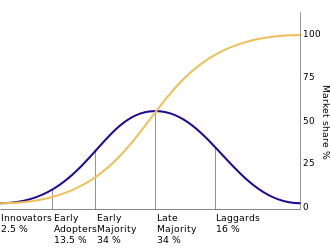
\includegraphics[width=0.80\textwidth]{pic_diffusion.png}
  \end{center}
  \caption{Zusammenspiel zwischen Personentypen und Innovation}
  WIKIPEDIA article DIFFUSION
  \label{pic_diffusion}
\end{figure}

\subsubsection{Personen}
Die für die Verhaltensausbreitung relevanten Personen eines sozialen Gefüges lassen sich in fünf Kategorien unterteilen, welche durch die Zeit, welche sie brauchen um eine neue Innovation zu akzeptieren, definiert werden. \cite{Rogers03}
\begin{enumerate}
\item \textbf{Innovatoren}: Innovatoren sind die ersten Personen innerhalb eines sozialen Netzwerkes, welche sich einer neuen Innovation annehmen und sie adaptieren. Diese Personen haben meist eine herausragende soziale oder intellektuelle Stellung innerhalb einer Gemeinschaft. Ihre Beziehungen reichen über sogenannte Weak Ties (Siehe Kap. \ref{intro_ties}) weit über das unmittelbare soziale Netz hinaus. Somit erfahren sie früher als andere von neuen Innovationen. Die initiale Adaption eines neuen Verhaltens durch einen Innovator, markiert auf der Zeitlinie welche in Abbildung \ref{pic_diffusion} dargestellt ist den Zeitpunkt $t_0$.
\item \textbf{Frühzeitiger Anwender}: Diese Personengruppe hat meist einen direkten Kontakt zu den Innovatoren und ist somit prädestiniert, ein Verhalten sehr Früh in der Zeitlinie einer Verhaltensausbreitung zu adaptieren. Der größte Unterschied zwischen den frühzeitigen Anwendern und den Innovatoren ist, dass sie, im Gegensatz zu Letzteren, bereits durch Observation innerhalb ihres sozialen Umfeldes sich zum Verhaltenswechsel entschlossen haben.
\item \textbf{Frühe und späte Mehrheit}: Diese beiden Klassen zusammen sind im Konzept der Personen eines sozialen Netzwerks mit Abstand die größte Gruppe. Die Unterscheidung zwischen früher und später Mehrheit ist rein zeitlicher Natur, da zwischen den Mitgliedern dieser Gruppe untereinander kein bemerkenswerter sozialer oder gesellschaftlicher Unterschied besteht.
\item \textbf{Nachzügler}: Nachzügler stehen am Ende der Kette und adaptieren ein neues Verhalten erst dann wenn fast schon das gesamte soziale Netz hin zu dieser Innovation gewechselt ist. Sie besitzen innerhalb einer Gesellschaft häufig einen niederen Stand oder verfügen über wenige soziale Verknüpfungen sowie eine geringe Innovationsbereitschaft. Unter realen Bedingungen kommt es selten vor, dass eine Innovation ein gesamtes soziales Netz vollständig gewinnen kann. Meist bleiben immer Personen übrig welche entgegen aller Vorteile an älteren Verhalten festhalten. Diese würden jedoch, da sie eine gegebene Innovation nie adaptieren, eine eigene Gruppe bilden. Denn der Begriff Nachzügler impliziert, dass spätestens zu einem Zeitpunkt $t_x >> t_0$, wenn auch spät, trotzdem adaptiert wird.
\end{enumerate}
\subsubsection{Kanäle der Verhaltensausbreitung}
\label{intro_ties}
Damit ein Individuum überhaupt auf die Idee kommt sein momentanes Verhalten durch ein neues zu ersetzen, muss als grundsätzliche Annahme gegeben sein, dass das Individuum von diesem neuen Verhalten über einen seiner Sinne Kenntnis genommen hat. Entweder er hat die Vorzüge des neuen Verhaltens selbst gesehen oder von einem Freund oder aus den Nachrichten davon gehört. Die Kanäle über welche sich die Information über eine neue Innovation verbreiten, sind so vielfältig das es den Rahmen dieser Arbeit sprengen würde, sie in großem Detail zu benennen. Allerdings biete sich die nähere Analyse von zwei Obergruppen an, über welche sich Informationen in sozialen Gemeinschaften verbreiten.
[Quelle Paper von Granovetter als Hauptquelle für diesen Abschnitt]
\paragraph{Strong Ties}
Unter Strong Ties (Starke Verknüpfungen) wird in einer Gemeinschaft die unmittelbare soziale Umgebung eines Individuums definiert. Diese besteht aus sehr nahen Verwandten, Bekannten und Freunden. Zu ihnen hat das Individuum eine sehr enge Verknüpfung, es schätzt ihre Meinung und meistens teilt es auch Verhaltensweisen sowie Interessen. Dies ergibt sich aus dem natürlichen Bestreben eines Individuums, sich mit Personen zu umgeben die ihm ähnlich sind. Strong Ties spielen bei der Verhaltensausbreitung die beherrschende Rolle, da hauptsächlich über sie die Verbreitung einer Innovation stattfindet, welche im Endeffekt zu einer Adaption führt. Es hat deutlich mehr Gewicht für ein Individuum, wenn einer seiner besten Freunde ein neues Verhalten adaptiert, als wenn es ein flüchtiger Bekannter tut. Während die Strong Ties folglich sehr förderlich für die Verhaltensausbreitung sind, so haben sie einen großen Nachteil was die pure Informationsverbreitung betrifft. Gerade weil die soziale Struktur innerhalb eines Netzwerks aus Strong Ties stark verknüpft ist gibt es darin wenig neue Information. Die Informationen welche ein Individuum von einem besten Freund oder nahem Verwandten bekommen kann hat es wahrscheinlich schon erfahren.
\paragraph{Weak Ties}
[KOMPLETT NEU SCHREIBEN MIT EINEM BILD ALS VERANSCHAULICHUNG]
\subsection{Zeit als Faktor}
Die Zeit als Faktor findet sich in drei Bereichen einer Verhaltensausbreitung wieder.
\begin{enumerate}
\item Der Entscheidungsfindungsprozess durchläuft entlang der Zeitachse mehrere Stufen in welchen sich das Individuum vom erstmaligen Hören einer Innovation bis hin zu dessen Adaption vorarbeitet. Wie schnell dies geschieht ist abhängig von den sozialen Strukturen und der Einstellung der Person selbst.
\item In welches Spektrum der Personen [LINK] ein Individuum zuzuordnen ist hängt maßgeblich davon ab, wann es sich dazu entscheidet eine Innovation anzunehmen. Während Innovatoren den Startschuss setzen entschließen Nachzügler sich erst sehr spät im Prozess der Verhaltensausbreitung eine Adaption in Betracht zu ziehen.
\item Der dritte Faktor ist definiert als die Rate der Adaption welche sich durch die Anzahl der Individuen berechnet, welche in einem gegebenen Zeitintervall ein neues Verhalten angenommen haben.
\end{enumerate}

\subsection{Historische Beispiele}
Eine der frühesten Studien zum Thema Verhaltensausbreitung wurde von Bryce Ryan und Neil Gross im US-Bundesstaat Iowa durchgeführt. Dieser im Midwesten der USA gelegene Staat ist besonders geprägt durch die dort vorherrschende Landwirtschaft, speziell dem Anbau von Mais. In ihrer Studie "Acceptance and Diffusion of Hybrid Corn Seed in two Iowa Communities" untersuchten Ryan und Gross wie, warum und über welche Wege ein neu entwickelter, bezüglich des Ertrags besserer, Hybridsamen Verbreitung fand. Dazu befragten sie mehrere Bauern wann sie damit begonnen hätten das neue Saatgut zu verwenden und wer sie auf die Idee dazu gebracht hatte. Ein Kernergebnis der Studie war, dass viele der Bauern bereits lange vor ihrer eigenen Adaption des neuen Saatguts, von seiner Existenz erfahren hatten. In den meisten Fällen durch Verkäufer welche natürlich versuchten das neue Produkt in den Markt einzuführen. Jedoch überzeugen ließen sich die meisten der Bauern erst zu dem Zeitpunkt als ein bekannter oder benachbarter Bauer sich dazu entschloss den Hybridsamen einzusetzen. Dies ist ein exemplarischer Fall für die Unterschiede zwischen Strong und Weak Ties. Über die Weak Ties (in diesem Fall die Verkäufer) trug sich lediglich die Innovation in das Netzwerk, allerdings nicht die Verhaltensausbreitung. Diese fand über die Mundpropaganda mit Bekannten und Nachbarn statt (Strong Ties). \\\\
Ein weiteres Beispiel welches Everett Rogers in seinem Buch Diffusion of Innovation beschreibt handelt von einem peruanischen Dorf in welchem die Regierung mittels eines Programms versuchen wollte, die Bewohner dazu zu bringen ihr Trinkwasser vor dem Konsum abzukochen. Viele Krankheitsfälle die eindeutig auf verschmutztes Trinkwasser zurückzuführen waren ließen die Regierung diesen Schritt nehmen. Dazu wurde in die Gemeinschaft eine Frau des Gesundheitsministeriums geschickt welche die ortsansässigen Hausfrauen schulen sollte. Das Projekt scheiterte nach mehreren Monaten damit, dass von allen Haushalten im Dorf lediglich drei das neue Verhalten angenommen hatten. Die Problematik hier lässt sich mit einer fehlenden Kompatibilität erklären. Die Einwohner (sowie ein Teil der gesamten peruanischen Bevölkerung) haben ein traditionelles Verständnis vom Konsum von heißen und kalten Getränken. Das Bild hierbei ist, dass nur kranke Menschen heiße Getränke zu sich nehmen. Somit stieß die Idee heißes (oder eigentlich nur zuvor abgekochtes) Wasser zu trinken auf massiven Widerstand da sie den herrschenden Normen nicht entsprach.

\section{Modellierung eines soziale Netzwerks}
Um die im vorherigen Abschnitt dargestellten, diffusen Aspekte eines realistischen sozialen Netzwerks für Analysezwecke zu verwenden, ist eine gewisse Abstraktion notwendig. Die Grundannahme besteht darin, dass jedes soziale Netzwerk ein Gebilde ist aus Personen, Verbindungen zwischen diesen Personen und Verhalten welche von ihnen angenommen werden können. Eine dafür sehr gut geeignete Repräsentation ist ein Graph dessen Knoten als Personen und Kanten als Verbindungen zwischen den Individuen dienen. Die verschiedenen Verhaltensweisen können als Attribute der Knoten interpretiert werden.\\\\

\begin{figure}
  \begin{center}
    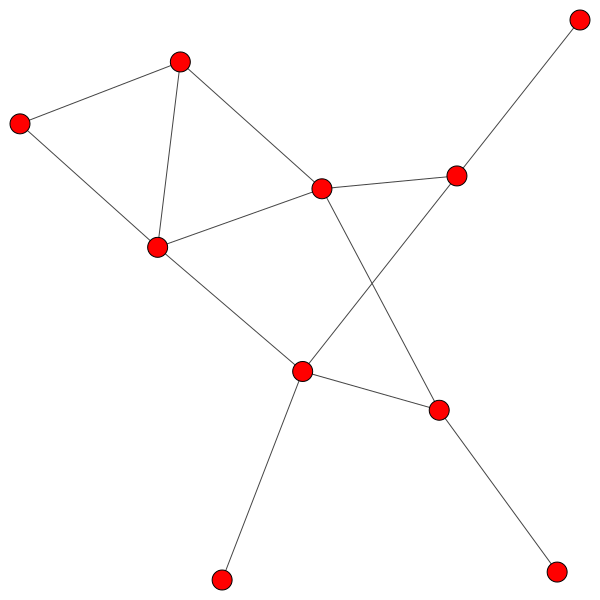
\includegraphics[width=0.60\textwidth]{pic_simpleGraph.png}
  \end{center}
  \caption{Ein einfacher ungerichteter Graph}
\end{figure}

Jedoch ist nicht jeder Graph automatisch geeignet um ein soziales Netzwerk, besonders im Bezug auf die Verhaltensausbreitung, zu repräsentieren. Die hierfür verwendeten Graphen müssen einer Reihe von grundlegenden Eigenschaften entsprechen.
\begin{enumerate}
\label{enum_graphConditions}
\item Der Graph muss zusammenhängend sein, was per Definition bedeutet, dass von jedem beliebigen Knoten des Graphen aus jeder beliebige andere Knoten über einen aus Kanten bestehenden Weg erreicht werden kann. Interpretiert darf man unter dieser Bedingung die Tatsache verstehen, dass jeder Mensch auf der Welt über eine endliche Anzahl an Verbindungen mit jedem anderen Menschen verknüpft ist. Studien zum Thema des "Small-World-Phenomena" beschäftigen sich weiterführend mit dieser These.
\item Der Graph muss ungerichtet sein. Diese Bedingung setzt als Grundlage die, vielleicht nicht immer vollends zutreffende, Annahme voraus, dass wenn ein Individuum A das Individuum B kennt, B ebenfalls der Existenz von A gewahr ist. Dies entspricht nicht immer exakt den reellen Bedingungen (Stalker, Prominente) aber ist für die Analyse solcher Netzwerke hinreichend annehmbar.
\item Der Graph muss die Eigenschaft der Irreflexivität besitzen. Angewandt auf die Analyse sozialer Netzwerke versteht man darunter, dass kein Knoten sein eigener Nachbar ist, ergo kein Individuum beeinflusst sich selbst bei seiner Entscheidung hin zu einem neuen Verhalten. Dafür wird über die Bedingung der Symmetrie nachdrücklich betont, dass wenn ein Knoten A der Nachbar von Knoten B ist, so ist auch B ein Nachbar von A.
\end{enumerate}


\subsection{Weak- und Strong Ties}
Wie im Kapitel \ref{intro_ties} bereits dargelegt, gibt es mit Strong- und Weak Ties zwei Obergruppen, in welche sich sämtliche Verbindungen innerhalb eines Netzwerkes klassifizieren lassen. Abbildung \ref{pic_ties} zeigt ein typisches, einfaches Beispiel für einen Graph mit klar erkennbaren Strong- und Weak Ties (starke Kanten sind Rot markiert und schwache Blau).\\
Klar identifizierbar sind hierbei die beiden eng verbundenen Gemeinschaften welche untereinander Strong Ties unterhalten. Hinüber zur jeweils anderen Gemeinschaft existiert nur ein einzelner Weak Tie. Dieser wird niemals effektiv für die Verhaltensausbreitung dienen aber, wie bereits diskutiert, potentiell die Information über neue Verhalten zwischen den Gemeinschaften austauschen.

\begin{figure}
  \begin{center}
    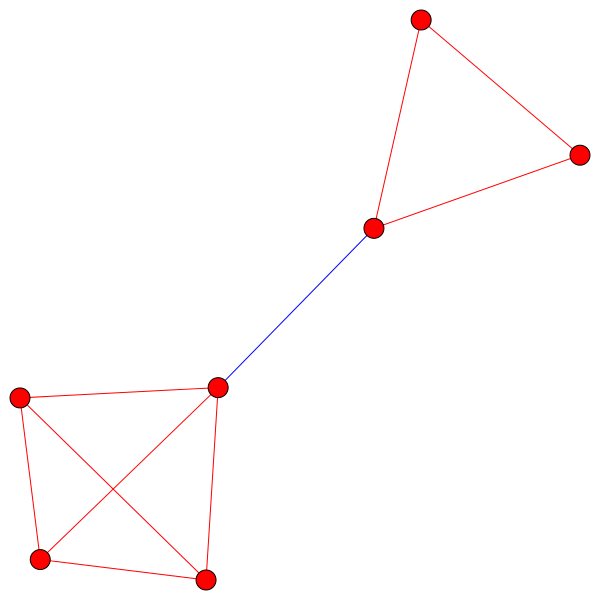
\includegraphics[width=0.60\textwidth]{pic_tieGraph.png}
  \end{center}
  \caption{Ein Graph mit hervorgehobenen Strong- und Weak Ties}
  \label{pic_ties}
\end{figure}

 

\section{Modellierung der Verhaltensausbreitung}
Nachdem die grundlegenden Bedingungen für die Modellierung eines sozialen Netzwerkes durch die Verwendung von bestimmten Graphen erfüllt sind, muss nun ein Modell gefunden werden, welches es erlaubt auf den genannten Graphen eine Verhaltensausbreitung zu simulieren.
\subsection{Networked Coordination Game}
Die Annahme der Verhaltensausbreitung besteht darin, dass jedes Individuum von der Adaption seines momentanen Verhaltens einen gewissen Nutzen hat welcher sich, unter Umständen abstrahiert, beziffern lässt. Nun stellt sich ihm die Möglichkeit ein neues Verhalten anzunehmen welches einen höheren Wert besitzt und somit einen klaren Vorteil sowie Anreizt es anstelle des alten zu adaptieren darstellt. Die Grundzüge dieser Idee spiegeln sich wieder in einem sogenannten "Networked Coordination Game". Hierbei haben die Spieler die Möglichkeit sich aus einer Auswahl an möglichen Verhalten ein beliebiges auszusuchen. Jedes Verhalten besitzt einen eigenen Payoff welcher mit dem Nutzen übersetzt werden kann welches dieses Verhalten für das Individuum bringt. Unter dieser ersten und vereinfachten Annahme wäre das Spiel schnell entschieden da sich jeder Spieler automatisch für das Verhalten mit dem höchsten Payoff entscheiden würde. Dies würde jedoch nicht den komplexen Verbindungen zwischen den Personen innerhalb eines Netzwerks Rechnung tragen und so muss eine Möglichkeit implementiert werden, dass die Payoffs eines Verhaltens abhängig sind von dem der unmittelbaren Nachbarn.\\\\ Die Darstellung der Payoffs in einer sogenannten "Payoff-Matrix" hilft dabei, die Idee zu veranschaulichen, dass der Nutzen eines Verhaltens auch davon abhängt was der Mitspieler als sein Verhalten gewählt hat. Tabelle \ref{my-label} stellt die Payoff-Matrix dar welche als Grundlage für die Verhaltensausbreitung dient. Die hier definierte Funktion $p$ legt fest was für einen Payoff Spieler eins und Spieler zwei beim Auswählen ihrer Verhalten beziehen. Sollten sich beide Spieler für das gleiche Verhalten entscheiden, so erhalten sie den jeweiligen Payoff. Bei einer heterogenen Entscheidung gibt es keine Punkte. Hiermit soll der Eigenschaft Rechnung getragen werden, dass wir stets einen Vorteil haben unser Verhalten dem unserer unmittelbaren Nachbarn anzupassen.
\begin{table}[h]
\centering
\caption{Exemplarische Payoff-Matrix}
\label{my-label}
\begin{tabular}{|l|l|l|l|}
\hline
                           & \multicolumn{3}{l|}{Spieler 1}          \\ \hline
\multirow{3}{*}{Spieler 2} &             & Verhalten A & Verhalten B \\ \cline{2-4} 
                           & Verhalten A & p(a,a)      & p(0,0)      \\ \cline{2-4} 
                           & Verhalten B & p(0,0)      & p(b,b)      \\ \hline
\end{tabular}
\end{table}

Die Payoff Matrix besitzt ebenfalls zwei sogenannte Nash-Equilibria (benannt nach dem berühmten Mathematiker John Nash) in den Fällen, dass beide Spieler sich für identische Verhalten entschieden haben. Per Definition des Nash-Equilibriums kann sich, ausgehend von diesen Situationen kein Spieler einen weiteren Vorteil verschaffen indem er allein sein Verhalten ändert.\\\\
Unter diesen Voraussetzungen wird jedoch noch nicht berücksichtigt, dass es in einem sozialen Netzwerk nicht nur zweier Pärchen gibt sondern ein Individuum sein Verhalten mit unter Umständen deutlich mehr Nachbarn abstimmen muss. Was bedeutet, dass in eine etwaige Kostenrechnung die bestimmt welches Verhalten lohnenswerter ist bei der Auswahl zwischen einem Verhalten A oder B, nicht nur allein deren Payoffs miteinbezogen werden dürfen. Auch die Anzahl der Nachbarn welche entweder das eine oder das andere Verhalten bereits adaptiert haben muss berücksichtigt werden.

 % 
 \begin{equation}
 \label{formel_payoffA}
 P_a = p*a*d
 \end{equation}
 %
  % 
 \begin{equation}
 \label{formel_payoffB}
 P_b = (1-p)*b*d
 \end{equation}
 %
 
 Formel \ref{formel_payoffA} zeigt die Berechnung des Payoffs $P_a$, welchen ein Individuum erhalten würde wenn es insgesamt $d$ Nachbarn besitzt und der Bruchteil $p$ davon sich bereits für das Verhalten A entschlossen hat. Formel \ref{formel_payoffB} stellt genau das gleiche dar nur ausgelegt für den Payoff $P_b$. Hier wird davon ausgegangen, dass es nur zwei unterschiedliche Verhalten A und B zur Auswahl gibt und jedes Individuum zwangsweise eines der beiden adaptiert haben muss. Dies gilt auch für das in obigem Beispiel erwähnte Individuum welches eine Entscheidung trifft. Es selbst kann beispielsweise B oder A adaptiert haben ohne, dass dies seine Entscheidung beeinflusst, da nach Definition in Auflistung \ref{enum_graphConditions} Niemand als sein eigener Nachbar zählt.
 %
  \begin{equation}
 \label{formel_payoffCompare}
 p*a*d \geq (1-p)*b*d
 \end{equation}
 %
Verhalten A wäre folglich die bessere Wahl wenn Formel \ref{formel_payoffCompare} erfüllt ist. Dabei gehen wir hier und in allen folgenden Beispielen davon aus, dass geprüft wird ob ein Netzwerk in dem initial alle Personen Verhalten B verwenden ein Wechsel hin zu Verhalten A möglich ist. Unter dieser Annahme wird dem Verhalten A auch der Vorteil gegeben, dass bei einem Gleichstand der beiden Payoffs $P_a$ und $P_b$ das Verhalten A adaptiert wird.
%
  \begin{equation}
 \label{formel_payoffFraction}
 p \geq \frac{b}{a+b}
 \end{equation}
 %
Formel \ref{formel_payoffFraction} erhält man durch Umformulierung der Formel \ref{formel_payoffCompare} und kann somit die Aussage treffen, dass wenn ein $p$ Bruchteil der Nachbarn eines Individuums das Verhalten A adaptiert haben, diese Person ebenfalls zu Verhalten A wechseln wird. Die Rechte Seite der Formel \ref{formel_payoffFraction} wird als Threshold bezeichnet und im weiteren Verlauf mit $q$ adressiert. Der Threshold ist, im homogenen Fall, für das gesamte Netzwerk identisch. Er beschreibt den Bruchteil an Nachbarn welche, abhängig von den Payoffs $a$ und $b$ mindestens nötig sind, um ein Individuum zur Adaption von Verhalten A zu bewegen.

\subsubsection{Heterogener Threshold}
Die Vorstellung, dass alle Personen innerhalb eines sozialen Netzwerks den gleichen Threshold besitzen, ist künstlich ideal und für eine einfache Analyse sehr dankbar, entspricht jedoch nur unzureichend der Realität. Unter dieser Bedingung könnte man beispielhaft davon ausgehen, dass wenn $50\%$ der Nachbarn eines Individuums Verhalten A adaptiert haben, wird diese Person ebenfalls wechseln. Allerdings ist jeder Mensch verschieden und besitzt somit seinen ganz individuellen Threshold. Manche lassen sich leichter beeinflussen und es genügen schon $30\%$ der Nachbarn um sie zum Wechsel zu bringen. Andere sind hartnäckiger und benötigen den Zuspruch von $80\%$ ihrer Nachbarn um alte Gewohnheiten aufzugeben. Diesen Umstand repräsentiert das hier vorgestellte Modell der Verhaltensausbreitung mit der Möglichkeit heterogene Thresholds zu verwenden.\\\\

Bei der Anwendung von heterogenen Thresholds besitzt nun jeder Spieler einen ganz eigenen Payoff für die beiden zur Verfügung stehenden Verhalten. Dies spiegelt sich auch in der Payoff Matrix für den Fall eines Networked Coordination Game mit heterogenen Thresholds wieder(\ref{table_payofHetero}.

\begin{table}[h]
\centering
\caption{Payoff Matrix mit heterogenen Thresholds}
\label{table_payofHetero}
\begin{tabular}{|l|l|l|l|}
\hline
                           & \multicolumn{3}{l|}{Spieler 1}           \\ \hline
\multirow{3}{*}{Spieler 2} &             & Verhalten A  & Verhalten B \\ \cline{2-4} 
                           & Verhalten A & p($a_1$,$a_2$) & p(0,0)      \\ \cline{2-4} 
                           & Verhalten B & p(0,0)       & p($b_1$,$b_2$)      \\ \hline
\end{tabular}
\end{table}

Somit besitzt jeder Knoten $k$ seinen individuellen Threshold $q_k$ dargestellt in Formel \ref{formel_thresholdHetero}.

%
  \begin{equation}
 \label{formel_thresholdHetero}
 q_k =  \frac{b_k}{a_k+b_k}
 \end{equation}
 %

\subsubsection{Beispiel mit homogenen Thresholds}
\label{sss_beispielHomo}
In den folgenden Bildern ist der Ablauf einer Verhaltensausbreitung in einem Netzwerk mit 10 Knoten sichtbar. Als Ausgangssituation ist das gesamte Netzwerk auf Verhalten B eingespielt (grün markiert). Ausgehend von einem zufällig gewählten initialen Adopter unter Berücksichtigung der Payoffs $a=2$ und $b=1$ kann für jeden Schritt separat nachvollzogen werden warum die einzelnen Knoten von Rot auf Grün gewechselt haben.


\begin{minipage}[t]{0.3\textwidth}
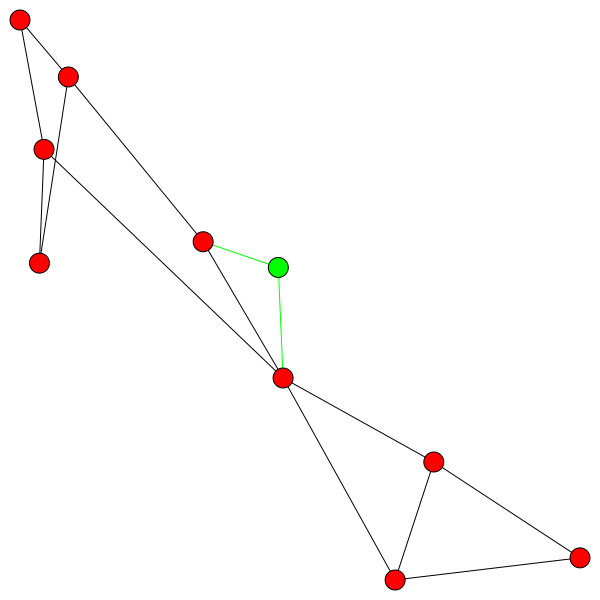
\includegraphics[width=\textwidth]{cascadeHomo/cascade.png}
\end{minipage}
\begin{minipage}[t]{0.3\textwidth}
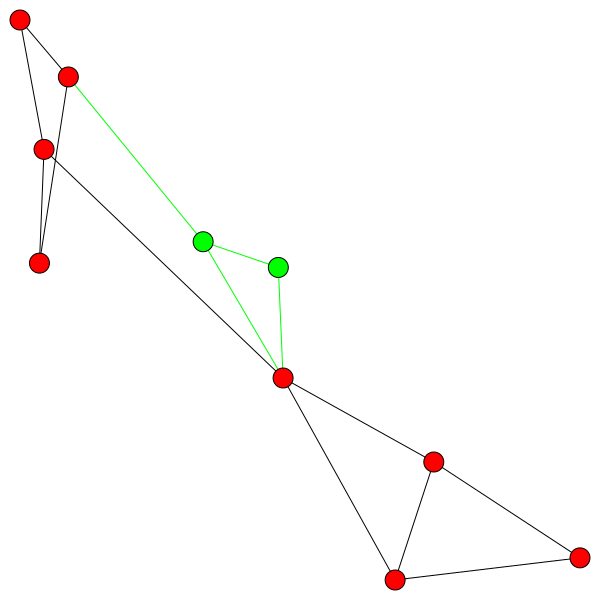
\includegraphics[width=\textwidth]{cascadeHomo/cascade0.png}
\end{minipage}
\begin{minipage}[t]{0.3\textwidth}
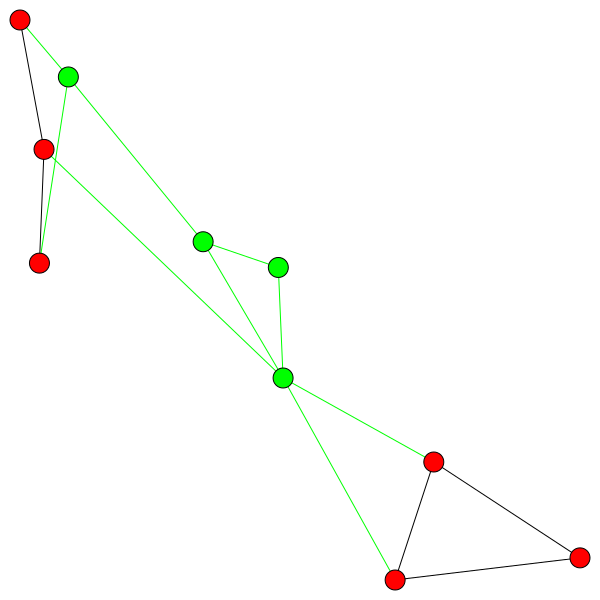
\includegraphics[width=\textwidth]{cascadeHomo/cascade1.png}
\end{minipage}
\begin{minipage}[t]{0.3\textwidth}
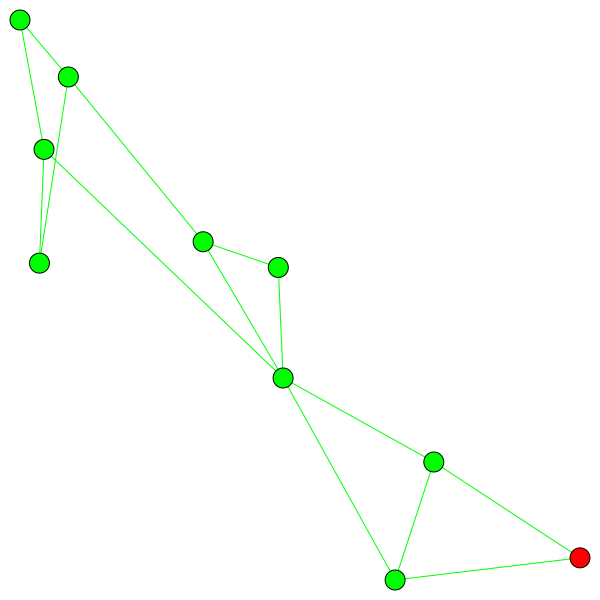
\includegraphics[width=\textwidth]{cascadeHomo/cascade2.png}
\end{minipage}
\begin{minipage}[t]{0.3\textwidth}
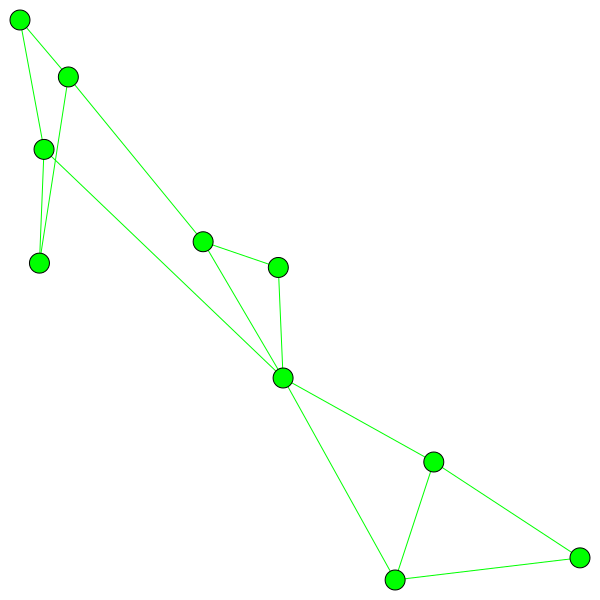
\includegraphics[width=\textwidth]{cascadeHomo/cascade3.png}
\end{minipage}
\begin{minipage}[t]{0.3\textwidth}
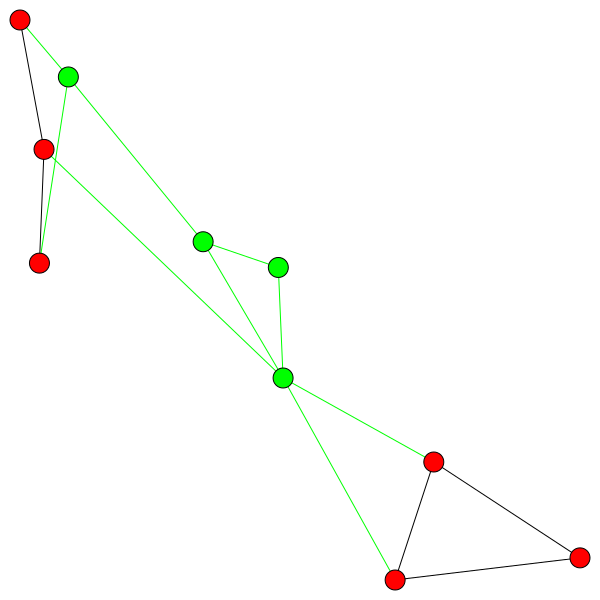
\includegraphics[width=\textwidth]{cascadeHomo/cascade1.png}
\end{minipage}

Exemplarisch wird dies anhand des Schritts fünf definiert wo man beobachten kann. [HIER BEISPIELHAFT EINEN SCHRITT DURCHSPIELEN MIT ANALYSE ZU ALLEN KNOTEN, DAFÜR SOLLTE ICH EINE GRAFIK AUSWERFEN WELCHE DIE KNOTEN MIT NUMERISCHEN LABELS VERSIEHT]

\subsection{Definition einer Kaskade}
Die im Kapitel \ref{sss_beispielHomo} zu beobachtende Kettenreaktion, wird im Rahmen der Verhaltensausbreitung als Kaskade bezeichnet. Der Begriff ursprünglich aus dem Französischen stammend ("`cascade"' - Wasserfall) wird auch im Deutschen verwendet, bei der Beschreibung von über mehrere Stufen abfallenden Wasserfällen. Diese Interpretation lässt sich nun direkt auf die Verhaltensausbreitung übertragen wo auch in mehreren Stufen (Steps) sich ein Verhalten immer weiter ausbreitet. Allgemein lässt sich von einer Kaskade sprechen, wenn in einem Netzwerk, welches den zuvor festgelegten Definitionen genügt, ausgehend von einem kleinen Kreis initialer Innovatoren, ein neues Verhalten nach und nach das gesamte Netzwerk erobert. Ist dieser Siegeszug absolut, also zum Endzeitpunkt $t_n$ einer Kaskade verwendet jeder Knoten das von ihr verbreitete Verhalten, spricht man von einer vollständigen Kaskade.
\subsection{Cluster als natürliche Hindernisse}
\label{ss_cluster}
Wie im vorherigen Kapitel bereits angesprochen wurde, ist es mitnichten garantiert, dass ausgehend von den initialen Adoptern, eine vollständige Kaskade entsteht. Gewisse Strukturen eines sozialen Netzwerks können die Ausbreitung einer Kaskade zum Stillstand bringen, gänzlich unabhängig von der Zeit (oder den Steps). Diese Strukturen werden Cluster genannt. Ein Cluster besteht aus einem Zusammenschluss von mehreren, eng verknüpften Knoten. Diese bilden ein verwobenes Geflecht, welches von innen her alle seine Mitglieder stark genug beeinflusst, um eine Einflussnahme von Außen potentiell auszuschließen.\\\\
Formal definiert lässt sich ein Cluster im Graph folgendermaßen beschreiben: \emph{Ein Cluster ist ein Zusammenschluss von Knoten innerhalb eines Graphen. Wenn für jeden Knoten innerhalb eines Clusters gilt, dass ein $x$-Bruchteil seiner Nachbarn sich ebenfalls innerhalb des Clusters befinden, so besitzt der Cluster die Dichte $x$}. Veranschaulichend lässt sich festhalten, dass jeder Knoten eines Graphen zusammengefasst ebenfalls einen Cluster der Dichte $1$ bildet.
[BILD MIT BEISPIEL EINES CLUSTERS]\\\\
Wenn nun eine Kaskade durch ein Netzwerk läuft welches einen Threshold $q$ besitzt und sich gleichzeitig in diesem Netzwerk ein Cluster mit einer Dichte $x > (1-q)$, so wird die Kaskade niemals vollständig werden. Da ein Knoten innerhalb des Clusters, gemäß des Thresholds, mindestens $q\%$ Nachbarn mit neuem Verhalten benötigt. Durch die Definition der Dichte des Clusters jedoch $x\%$ der Nachbarn innerhalb des Clusters sind, also per se selbst noch das alte Verhalten benutzen ohne Chance das neue zu adaptieren. Somit können die Knoten außerhalb des Clusters niemals die nötige Mehrheit erlangen um den Knoten innerhalb zum Umschwenken zu bewegen. \\\\
Cluster sind folglich die natürlichen und auch einzigen Hindernisse von Kaskaden. Gelingt es einer Kaskade nicht ein Netzwerk vollständig zum Umschwenken zu bewegen, dann lässt sich direkt daraus schließen, dass dieses Netzwerk einen Cluster mit der Dichte $x > (1-q)$ enthält.

 
\subsection{Kapazität einer Kaskade}
Der Threshold eines Netzwerkes ist, ersichtlich aus Formel \ref{formel_payoffFraction} abhängig von den beiden Payoffs $a$ und $b$. Um den Threshold $q$ abzusenken, um beispielsweise das dichte Netz eines Clusters vielleicht doch durchdringen zu können, bieten die beiden Werte $a$ und $b$ einen gewissen Spielraum. Jedoch ausgehend von der Annahme, dass man bestrebt ist das Verhalten $A$ innerhalb eines Netzwerks zu verbreiten, verringert sich dieser Spielraum lediglich noch auf den Faktor $a$ (da man keinen Einfluss auf das vorherrschende Verhalten $B$ hat). Dieser Faktor $a$ muss erhöht werden um ein Absinken des Thresholds zu bewirken. Angewandt auf die Realität könnte dies bedeuten, dass eine Firma ihr Produkt mit weiteren Investitionen verbessert um seine Qualität zu erhöhen und damit den Payoff zu steigern. Allerdings besteht hierbei die Gefahr, dass man zu viel investiert und das Produkt sich vielleicht auch mit einem niedrigeren Payoff und weniger kostspieligen Investitionen am Markt durchgesetzt hätte.\\
An diesem Punkt wird die sogenannte Kapazität einer Kaskade interessant. Diese ist eine gegebene Eigenschaft eines jeden individuellen Graphen und wird definiert durch den höchst möglichen Threshold q (und damit verbunden dem kleinsten, billigsten Payoff a) für welchen eine Kaskade ein Netzwerk vollständig erobern kann.\\\\
Um dies korrekt analysieren zu können, müssen zunächst weitere Bedingungen für den Graphen angenommen werden. Die Auswahl der Innovatoren muss so gewählt werden, dass ihre Anzahl stets deutlich kleiner ist als die gesamte Anzahl an Knoten. Bei der Betrachtung Netzwerk mit $100$ Knoten von denen $90$ Innovatoren sind, würde man kaum relevante Ergebnisse bezüglich der Verhaltensausbreitung beobachten können. Für den allgemeinen Fall legt man deswegen für das Netzwerk fest:
\begin{enumerate}
\item Das Netzwerk besteht aus unendlich vielen Knoten.
\item Jeder Knoten hat nur endlich viele Nachbarn.
\item Die Anzahl $I_0$ der Innovatoren ist endlich.
\end{enumerate}
Alle zuvor festgelegten Bedingungen für den Graphen gelten auch weiterhin. Damit ist die Grundlage für die Analyse der Kapazität einer Kaskade gestellt.
\subsubsection{Kapazität des infiniten Pfades}
Eine der einfachsten Netzwerkstrukturen ist der infinite Pfad [BILD]. Wenngleich seine Ausdehnung, gemäß der im vorherigen Abschnitt festgelegten Definition, unendlich in beide Richtungen geht, genügt bereits ein einzelner Innovator $v_i$ um die Kapazität dieses Netzwerks zu demonstrieren. Zudem ist die Bewegung der Kaskade nach links und rechts entlang des Pfades, ausgehend von $v_i$, identisch. Somit genügt es vollkommen nur eine Seite zu betrachten.\\
Ausgehend von einem beispielhaften Threshold von $30\%$ würde sich die Kaskade vollständig ausbreiten da für die unmittelbaren Nachbarn von $v_i$ die Bedingung des Thresholds mehr als erfüllt ist ($50\% > 30\%$). Es ist an dieser Stelle nun trivial ersichtlich, dass die Kapazität der Kaskade eines infiniten Pfades $\frac{1}{2}$ beträgt. Für größere Threshold Werte wird die Kaskade niemals über $v_i$ hinaus Verbreitung finden. Wenngleich auch $\frac{1}{2}$ natürlich nicht für alle Netzwerke gilt (das infinite Gitter beispielsweise hat die Kapazität $\frac{3}{8}$) so stellt $\frac{1}{2}$ doch einen Sonderfall dar. Denn dieser Wert ist die maximal mögliche Kapazität einer Kaskade für ein Netzwerk das allen bisher gestellten Bedingungen gerecht wird. Den Beweis hierzu liefern Easly und Kleinberg \cite{Easly10}. 

\subsection{Bilinguale Option}
Wenngleich es natürlich das oberste Ziel bei der Verhaltensausbreitung ist, eine vollständige Kaskade zu erzeugen, so ist dieser Ausgang unter halbwegs realistischen Bedingungen doch eher selten. Meist stellt sich ab einem gewissen Punkt der Ausbreitung einer Kaskade ein Gleichgewicht zwischen den beiden Verhalten ein in dem beide koexistieren.\\\\
Ein gutes Beispiel hierfür ist die Ausbreitung von Sprachen in Ländern. Die Deutschen sprechen Deutsch und die Franzosen sprechen Französisch. An diesem Zustand wird sich nicht einfach zufällig etwas ändern, sprich der deutschen Sprache wird nie die Ausbreitung in den Cluster Frankreich gelingen und vice versa. Allerdings lässt sich nun an den Grenzen zwischen den beiden Verhalten (oder den beiden Ländern) das Phänomen der bilingualen Option beobachten. Die Menschen in Luxemburg sprechen weder ausschließlich Deutsch noch Französisch. Stattdessen haben sie sich für eine dritte Möglichkeit entschlossen, beide Sprachen zu sprechen, um bei der Kommunikation einen Vorteil mit beiden Nachbarn zu haben.

\begin{table}[h]
\centering
\caption{Payoff Matrix mit bilingualer Option}
\label{table_payoffBi}
\begin{tabular}{|l|l|l|l|l|}
\hline
                           & \multicolumn{4}{l|}{Spieler A}                                          \\ \hline
\multirow{4}{*}{Spieler B} &    & A     & B     & AB                                                 \\ \cline{2-5} 
                           & A  & $(a,a)$ & $(0,0)$ & $(a,a)$                                              \\ \cline{2-5} 
                           & B  & $(0,0)$ & $(b,b)$ & $(b,b)$                                              \\ \cline{2-5} 
                           & AB & $(a,a)$ & $(b,b)$ & $((a,b)^+$, $(a,b)^+)$ \\ \hline
\end{tabular}
\end{table}

Diese zusätzlich Option lässt sich in der Payoff Matrix (Tabelle \ref{table_payoffBi}) auslesen. Hieraus ist ersichtlich, dass ein Individuum mit adaptiertem Verhalten $AB$ von beiden Verhalten bei seinen Nachbarn profitiert. Die Notation $(a,b)^+$ für den Fall eines Nachbarn welcher ebenfalls $AB$ adaptiert hat, bedeutet, dass in diesem Fall der höhere Payoff von beiden genommen wird.


\section{Simulation einer Kaskade mit Igraph und Python}
Mal fragen ob er diese Sektion drin haben will oder ob das nicht in die Arbeit gehört. Ansonsten hier einfach ein wenig beschreiben wie die einzelnen Tools im zusamenspiel verwendet wurden mit dem ein odere anderen RAtschlag oder Screenshot, könnte vielleicht der nützlichste Teil werden wenn sich hinterher nochmal jemand damit beschäftigen will.

\section{Virales Marketing}
Möglichkeiten die Ausbreitung eines Verhaltens in einem Netzwerk künstlich zu stützen oder hervorzuheben. Besonders im Bezug auf Werbung oder Trends die Künstlich gesetzt werden wollen bauen Firmen zunehmends darauf, dass die sozialen Netzwerke für die Verbreitung genutzt werden. Das hängt besonders mit dem im Kapitel Verhaltensausbreitung bereits besprochenen Umstand zusammen, dass wir die Meinung eines uns näher stehenden Menschen mehr schätzen. Daher werden auch gerne Prominente für Werbung verwendet, zwar kennen wir sie nicht persönlich aber haben schon einmal von ihnen gehört und eine Meinung über sie. Ist diese Meinung gut dann vertrauen wir dem was sie sagen schon einmal intuitiv mehr als wenn und Dr Best eine neue Zahnbürste empfiehlt.
\subsection{Change Agents}
Wenn in Clustern bestimmte Seeds gesetzt werden sollen ist es von großem Vorteil Personen dafür auszusuchen die eine sehr starke Position im sozialen Gefüge haben. Als Alternative zu dem vorherig genannten Muster können auch anstatt die Brücke zu überwinden in dem neuen Netzwerk einflussreiche Personen gekauft werden damit diese als INnovatoren sich hervortuen und das Produkt den anderen empfehlen. Wieder ein Faktor warum Justin Bieber mit 50 mio Twitter followern ein beliebter Werbeträger ist. Wenn er etwas twittert sehen das direkt millionen von Menschen. 
\subsection{Beispiele für Virales Marketing}
Mit Bezug auf die neue Arbeit über Kaskadeneffekte in sozialen Medien, dass auch wenn diese auf den ersten Blick prädestiniert für einen solchen Einsatz wirken, sie nicht immer den gewünschten Erfolg erzielen. 

\section{Fazit}
Knappes Fazit darüber was die Erkenntnisse und Ergebnisse der Arbeit sind, im Bezug auf die vorgestellten Arbeiten, dass diese auch trotz ihres Alters immer noch große Relevanz haben und sich die in ihnen befindlichen Inhalte auch auf neuere Medien übertragen lassen können. Verhaltensausbreitung wird immer ein Teil der Zwischenmenschlichen Dynamik bleiben und somit auch die Forschung darüber nachfolgende Arbeiten beschäftigen.


\begin{thebibliography}{9}

\bibitem{morris98}
  Stephen Morris:
  \emph{Contagion},
  Yale University,
  1998.
 
\bibitem{strang98}
	David Strang, Sarah A. Soule:
	\emph{Diffusion in Organisations},
	Annu. Rev. Sociol., 1998, pp. 265-290.
	
\bibitem{Easly10}
	David Easly, John Kleinberg: 
	\emph{Networks, Crowds and Markets},
	Cambridge University Press, 2010, pp. 561-603.
	
\bibitem{Rogers03}
	Everett M. Rogers: \emph{Diffustion of Innovation}, Fifth
	Edition, Free Press, 2003
	
\bibitem{Ryan43} Bryce Ryan, Neil Gross: \emph{Acceptance and 		    Diffusion of Hybrid Corn Seed in Two Iowa Communities}, Agricultural Experiment Station Iowa State College of Agriculture and Mechanic Arts, 1950
\end{thebibliography}



\end{document}